\documentclass[../main.tex]{subfiles}
\graphicspath{{\subfix{../images/}}}
\begin{document}

Camera intrinsic parameters describe the internal geometry of the camera and define how three-dimensional points are projected onto the two-dimensional image plane.  
They are governed by the optical pathway through the lens and determine how real-world distances correspond to image pixel coordinates.  
The intrinsic model is typically divided into an idealized pinhole projection and a lens distortion model.

Under the pinhole model, the projection of a point onto the image plane is given by the intrinsic matrix:

\begin{equation}
    \mathbf{K} = 
    \begin{bmatrix}
        f_x & s & c_x \\
        0 & f_y & c_y \\
        0 & 0 & 1
    \end{bmatrix},
\end{equation}

where $(f_x, f_y)$ are focal lengths in pixels, $(c_x, c_y)$ denotes the principal point, and $s$ represents the skew factor (generally $s=0$ for modern sensors).

Real lenses introduce distortion, primarily radial, due to refraction near the outer edge of the lens.  
This effect, most pronounced in wide-angle optics, causes straight lines to appear curved.  
Radial distortion is modeled using polynomial coefficients $k_1$, $k_2$, and $k_3$:
\begin{equation}
    \begin{split}
        x' &= x_n(1 + k_1 r^2 + k_2 r^4 + k_3 r^6), \\
        y' &= y_n(1 + k_1 r^2 + k_2 r^4 + k_3 r^6),
    \end{split}
\end{equation}

where $(x', y')$ are distorted coordinates, $(x_n, y_n)$ are ideal coordinates, and $r = \sqrt{x_n^2 + y_n^2}$ is the radial distance from the optical center.  
Although this model omits asymmetric distortions, high-quality lenses typically minimize such effects.  
Even with manufacturer-provided parameters, recalibration ensures sub-pixel accuracy when aligning \ac{LiDAR} projections with image data.

To estimate intrinsic parameters, a planar checkerboard with known square dimensions is imaged from multiple orientations and distances.  
Its grid of high-contrast corners serves as stable reference points for gradient-based corner detection algorithms such as the Harris method.  
Calibration software uses these detected points to compute statistically optimal parameters across the full image set.

Effective calibration requires dozens of images taken at diverse depths and orientations spanning the camera’s operational field of view.  
Checkerboard dimensions should approximate the scale of observed objects to ensure that the chosen camera provides adequate spatial resolution (as discussed in Section~\ref{camera_selection}).  
Following these practices produces robust intrinsic estimates across the full imaging range.

% \begin{figure}[htbp]
% \centering
% \makebox[\textwidth][c]{%
%     \begin{subfigure}[t]{0.3\textwidth}
%         \centering
%         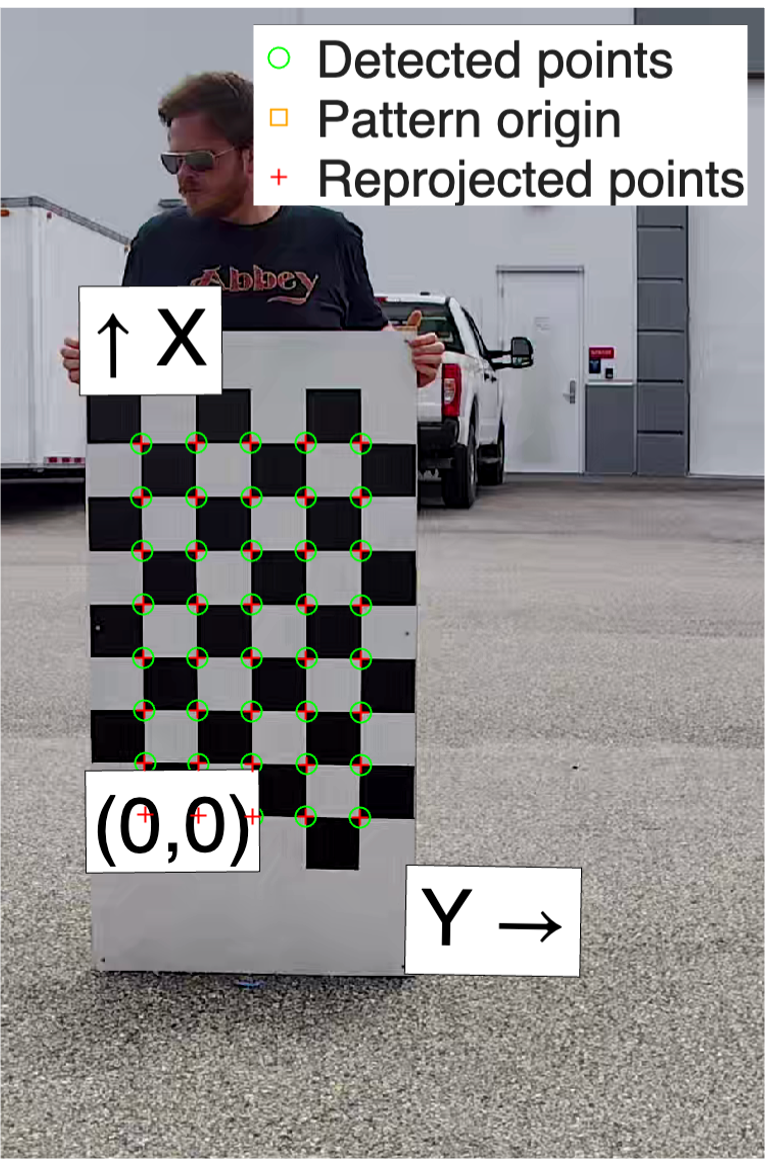
\includegraphics[width=\textwidth]{Images/cam_calib_1.png}
%         \caption{A single example of detected and reprojected checkerboard corners. Agreement between detected (green circles) and reprojected (red crosses) points demonstrates corner localization and mapping of the image coordinate system.}
%         \label{fig:cam_calib_1}
%     \end{subfigure}
%     \hspace{2em}
%     \begin{subfigure}[t]{0.625\textwidth}
%         \centering
%         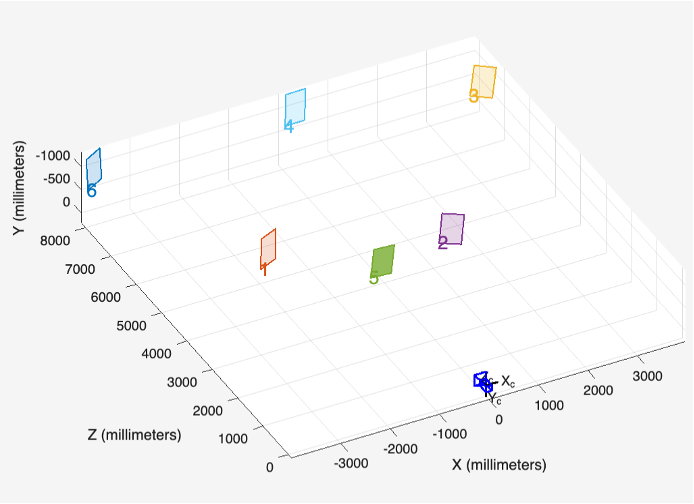
\includegraphics[width=\textwidth]{Images/cam_calib_2.png}
%         \caption{Reprojection of sample target poses into the 3D world frame after calibration.}
%         \label{fig:cam_calib_2}
%     \end{subfigure}%
% }
% \caption{Checkerboard images are processed to detect corners (left), which enable intrinsic parameters to be estimated and validated by reprojecting known targets into 3D space (right).}
% \label{fig:cam_calib}
% \end{figure}

\end{document}